\documentclass{ieeeaccess}
\usepackage{cite}
\usepackage{amsmath,amssymb,amsfonts}
\usepackage{algorithmic}
\usepackage{graphicx}
\usepackage{textcomp}
\usepackage{xcolor}
\usepackage{array}
\emergencystretch=3em

% Gerado por paper/build_tex.py a partir dos resultados em results/; não editar números à mão.
\begin{document}

\history{Date of publication xxxx 00, 0000, date of current version xxxx 00, 0000.}
\doi{10.1109/ACCESS.2017.DOI}

\title{Do Large Language Models Improve Adaptive Normative Agents? Norm Adaptation and Norm Compliance in Paired Simulations}
\author{\uppercase{Marx Viana}\authorrefmark{1},
\uppercase{Elder Cirilo}\authorrefmark{2},
\uppercase{Paulo Alencar}\authorrefmark{3},
\uppercase{Donald Cowan}\authorrefmark{3},
\uppercase{Carlos Lucena}\authorrefmark{1}}

\address[1]{Pontifical Catholic University of Rio de Janeiro, Rio de Janeiro, Brazil \{mleles, lucena\}@inf.puc-rio.br}
\address[2]{Federal University of São João del Rei, Minas Gerais, Brazil \{elder\}@ufsj.edu.br}
\address[3]{David R. Cheriton School of Computer Science, University of Waterloo, Waterloo, Ontario, Canada \{palencar, dcowan\}@uwaterloo.ca}

\tfootnote{This work was supported by the Brazilian funding agencies CAPES, CNPq and the Natural Sciences and Engineering Research Council of Canada (NSERC)}

\markboth
{Viana \headeretal: Do LLMs Improve Adaptive Normative Agents?}
{Viana \headeretal: Do LLMs Improve Adaptive Normative Agents?}

\corresp{Corresponding author: Marx Viana (e-mail: mleles@inf.puc-rio.br).}

\begin{abstract}
Large language models are increasingly proposed as reasoning components of normative multi-agent systems, yet their benefit over deterministic alternatives is rarely measured. We report two exploratory, controlled studies on an open platform in which every language-model component has a deterministic counterpart and all conditions are paired by seed and independent of agent order. The first study uses language models to adapt norms in a book marketplace, an intensive care alarm system and software project management. Language-model agents completed more trades, and adaptive norms reduced false alarms by 66\%, but a language-model norm recommender was worse than a deterministic one, and a language-model decision agent only matched a clinical early-warning score. The second study lets the alerting agent decide whether to comply with each alarm obligation under imperfect enforcement. A selfish strategy guided by the clinical score removed more false alarms than norm adaptation without harming patients, whereas a rebellious strategy delayed the recognition of deterioration; a regimented critical norm bounded the harm. The language-model agent suppressed 23\% of regulated alarms when detection was unlikely and almost none when it was certain, never suppressed a real deterioration and never harmed a patient. Its stated beliefs were cautious and always coherent with its decisions, but for the same alarms they shifted with the probability of detection, so its justifications partly rationalize its choices. We also report seventeen engineering threats to validity and their controls. With three seeds per condition, all findings are exploratory.
\end{abstract}

\begin{keywords}
enforcement, large language models, MAPE-K, multi-agent systems, norm compliance, normative systems, self-adaptive systems, simulation, threats to validity
\end{keywords}

\titlepgskip=-15pt

\maketitle

\section{Introduction}\label{sec:1}
Multi-agent systems (MAS) operating in regulated domains are typically governed by \emph{norms}—obligations, prohibitions and permissions with associated sanctions and rewards \cite{lopez2002constraining}. Our earlier work proposed the ANA metamodel and the ANA-ML modeling language to represent adaptive normative agents explicitly \cite{viana2022creating,viana2017modeling}, and the JSAN framework to implement them \cite{viana2015jsan}. Norms in such systems are usually static: thresholds, deadlines and scopes are fixed at design time, which is problematic when the environment changes or when one norm must serve heterogeneous contexts.

Large Language Models offer a tempting remedy. LLM-based agents can encapsulate the analysis, planning and knowledge stages of the MAPE-K loop \cite{nascimento2023selfadaptive,kephart2003vision}, and LLM components can interpret natural-language norms, recommend refinements, validate candidate norms and audit their effects. ANA-ML 2.0 proposes exactly these constructs—LLM-NormProcessor, LLM-NormRecommender, LLM-NormValidator and LLM-NormAuditor—and motivates them with an ICU patient-monitoring case in which adaptive norms should reduce false alarms and response times \cite{viana2025anaml2}.

Such expectations are hard to verify. LLM agents are stochastic and costly to run; simulations of interacting agents contain subtle sources of bias; and a fair comparison requires a non-LLM baseline that receives exactly the same information. In practice, it is easy to obtain impressive numbers from a setup that silently favors one condition. This paper reports an exploratory, controlled study designed to avoid these pitfalls. Our main findings are:

\begin{itemize}
\item In open negotiation, LLM agents completed twice as many trades as heuristic agents (2 vs. 1 per run) at higher prices, and did not exhibit the self-messaging behavior reported in earlier LLM-MAS experiments \cite{nascimento2023selfadaptive}.
\item Adaptive norms reduced ICU false alarms by 66\%, but the gain came from adaptation itself: the LLM-NormRecommender produced +27 false alarms per run relative to a deterministic recommender, because it adapted less under uncertain labels.
\item An LLM decision agent was as accurate as a NEWS2-based clinical score, not better, and adaptation increased alarm latency rather than reducing it.
\item Nine engineering threats to validity—order bias, off-by-one measurement, ground-truth leakage, ambiguous command semantics and others—would each have distorted the comparison had they gone unnoticed; two were first revealed by the LLM-NormAuditor itself.
\end{itemize}

Study 1 treats the LLM as a component \emph{of} the norms—recommending, validating and auditing them. The ANA metamodel, however, also allows agents to decide \emph{not} to comply with a norm when its rewards and punishments do not justify it \cite{viana2022creating}. Study 2 therefore asks a complementary question: rather than adapting a norm to reduce alarm fatigue, can an autonomous agent \emph{deviate} from it, and what does deviation cost? We compare five classical compliance strategies \cite{lopez2002constraining} with an LLM deliberative agent under different enforcement levels. Its main findings are:

\begin{itemize}
\item Well-informed deviation outperformed norm adaptation offline: a selfish strategy suppressing only alarms judged false by NEWS2 left 42.7 false alarms per run (adaptation: 74.0) with no harmed episode and unchanged latency.
\item Uninformed deviation was costly: a rebellious strategy harmed 4.0 episodes per run and more than doubled alarm latency; the regimented critical norm was the safety net.
\item Enforcement separated the strategies as theory predicts: opportunistic agents responded to detection probability, pressured agents to the expected sanction.
\item The LLM deliberative agent was safe but cautious: it suppressed 22.8\% of regulated alarms at p = 0.3 and 0.3\% at p = 1.0, all of them false, and harmed no patient; it thus removed far fewer false alarms (163.7 left) than a selfish agent guided by a clinical score.
\item Its stated beliefs were always coherent with its decisions, yet for the very same alarms they moved with the detection probability (45 beliefs changed from ``real'' to ``false'' and 15 the other way between p = 0.3 and p = 1.0; exact McNemar p = 0.0001): LLM justifications partly rationalize the decision rather than report an independent judgment.
\end{itemize}

Our contributions are: (i) \emph{llm-mas}, an open platform in which every LLM component has a deterministic counterpart, enabling paired comparisons; (ii) an evidence model for ICU alarms with imperfect, noisy observations, a clinical-score baseline and a Bayes-optimal ceiling; (iii) an empirical comparison across three scenarios; (iv) an operationalization of the ANA normative process with classical compliance strategies, imperfect enforcement and a regimented safety norm, compared with an LLM deliberative agent; and (v) a catalog of engineering threats to validity for LLM-based MAS simulations, with the controls we adopted. Section~\ref{sec:2} presents the background, Section~\ref{sec:3} the design of both studies, Sections~\ref{sec:4} and \ref{sec:5} their results, Section~\ref{sec:6} the implications, Section~\ref{sec:7} the threats to validity, and Section~\ref{sec:8} concludes.

\section{Background}\label{sec:2}
\subsection{Adaptive normative agents}\label{sec:2.1}
Following López y López et al. \cite{lopez2002constraining} and the ANA metamodel \cite{viana2022creating}, a norm is characterized by its \emph{addressee} (agents or roles responsible for it), \emph{deontic concept} (obligation, prohibition or permission), \emph{activation} and \emph{expiration} conditions, the \emph{state} or action it regulates, and the \emph{rewards} and \emph{punishments} associated with fulfilling or violating it. ANA extends the TAO and FAML metamodels \cite{beydoun2009faml,dasilva2004conceptual} with adaptation entities—Collect (sensors), Analyze (strategies), Decision (plans) and Effector (actuators)—and with a normative process in which agents become aware of norms, deliberate about them, decide whether to comply, and update their goals. ANA-ML represents these concepts as a UML-based language \cite{viana2022creating,viana2017modeling}; JSAN provides an implementation framework \cite{viana2015jsan}.

Fig.~\ref{fig:1} shows the ANA-BDI architecture that operationalizes this process \cite{viana2022creating}. A \emph{normative component} holds the norms beside the agent's beliefs, desires, intentions and plans; an \emph{adaptive component} runs a Collect–Analyze–Decision–Effector loop. Collect monitors and adopts norms; Analyze conditions them, verifies whether they are being fulfilled, estimates their \emph{normative contribution} to the agent's goals and detects and solves conflicts; Decision weighs the importance of the available options and selects a plan; and the Effector carries out the normative decision—which may be to fulfill the norm or to violate it. The separation between Analyze, which forms judgments, and Decision, which chooses, matters for Study 2: it is where an LLM can be placed, and it is what our analysis of LLM beliefs and decisions probes.

\begin{figure}[!t]
\centering
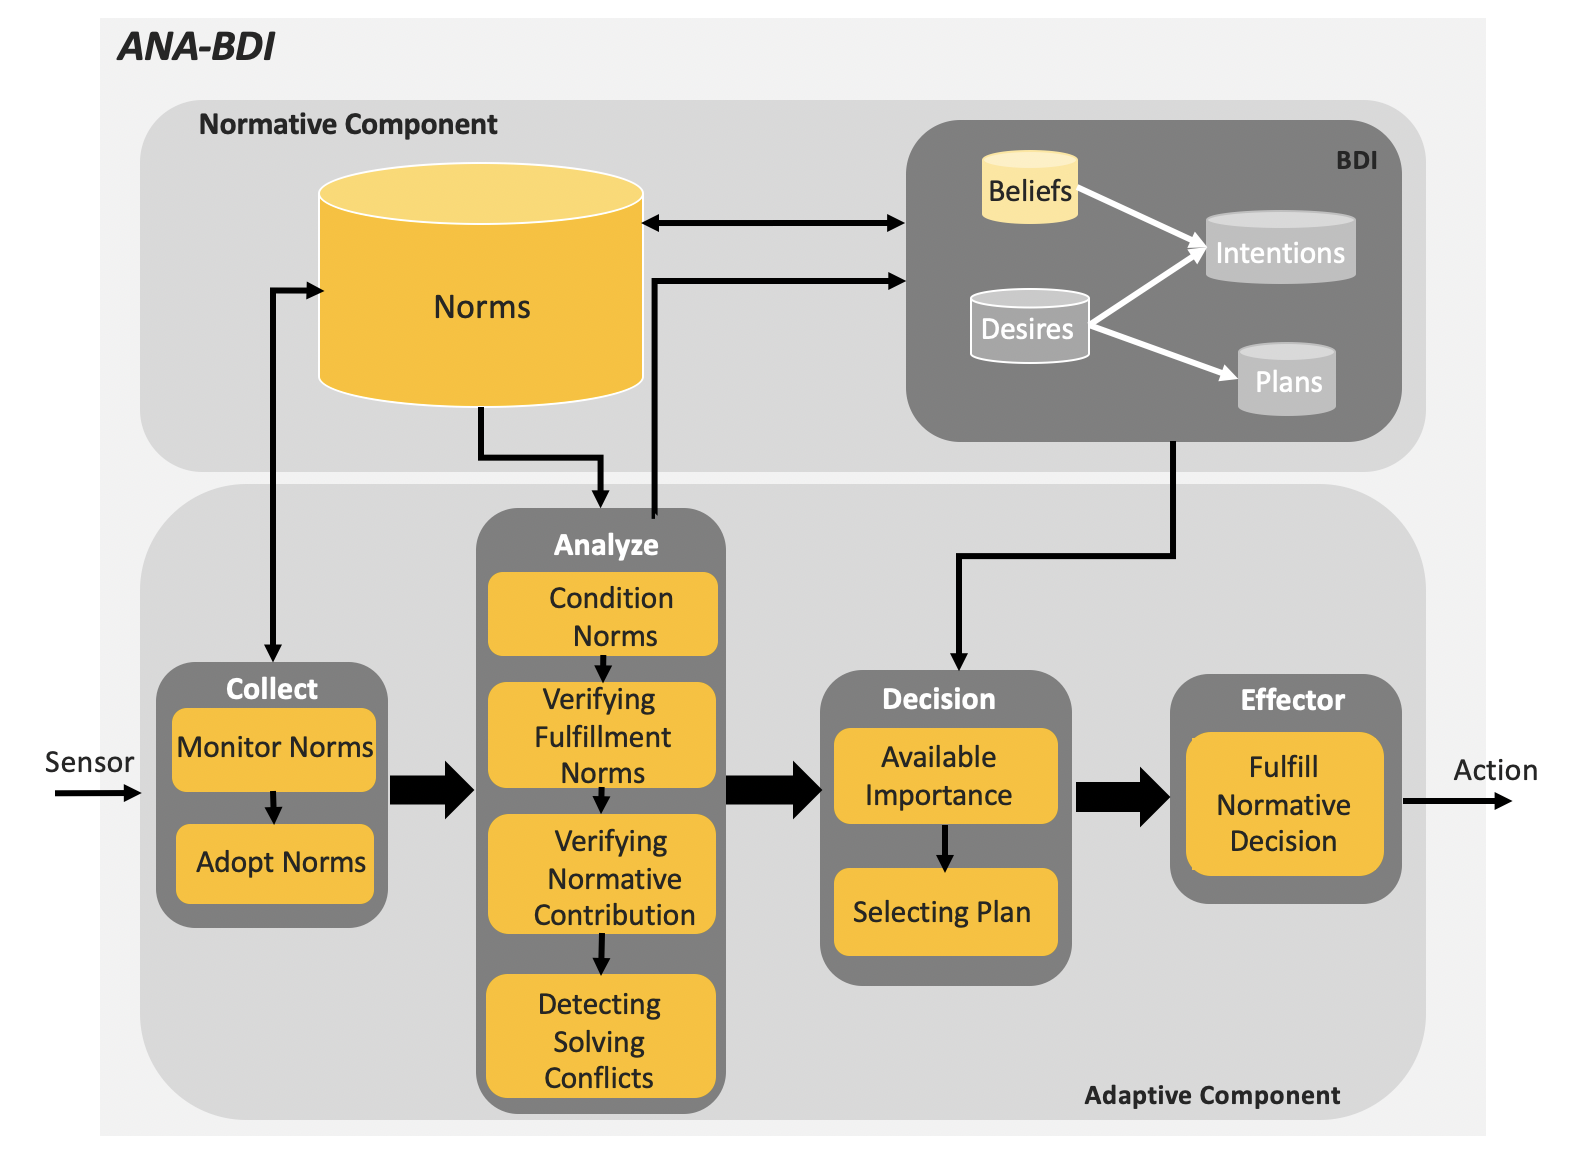
\includegraphics[width=\columnwidth]{figures/viana1.png}
\caption{ANA-BDI architecture of an adaptive normative agent (reproduced from \cite{viana2022creating}). Study 2 maps the alarm obligations, the deliberation and the alarm decision onto its Collect, Analyze, Decision and Effector stages.}
\label{fig:1}
\end{figure}

\subsection{LLM-based self-adaptive agents}\label{sec:2.2}
Nascimento, Alencar and Cowan \cite{nascimento2023selfadaptive} proposed agents whose MAPE-K loop \cite{delemos2013roadmap,kephart2003vision} delegates Analyze, Plan and Knowledge to an LLM: the Monitor stage turns sensors and received messages into a prompt, and the Execute stage parses the LLM output into actions. In a book marketplace with sellers and buyers, they observed both effective negotiation and undesired behaviors, such as an agent sending messages to itself while impersonating a customer, and they identified the lack of memory across iterations as a limitation.

\subsection{LLM components for norm adaptation}\label{sec:2.3}
ANA-ML 2.0 \cite{viana2025anaml2} introduces LLM-based constructs for continuous norm adaptation: an \emph{LLM-NormRecommender} proposes context-aware refinements; an \emph{LLM-NormValidator} checks consistency and conflicts; an \emph{LLM-NormAuditor} reports on norm effectiveness in natural language; and a human-in-the-loop supervisor approves changes. Its motivating case is ICU monitoring, where static alarm thresholds produce alarm fatigue. Clinical practice offers a strong non-LLM reference for alarm triage: the National Early Warning Score 2 (NEWS2) \cite{rcp2017news2}, which aggregates points for vital signs and level of consciousness, with a dedicated SpO\textsubscript{2} scale for patients with hypercapnic respiratory failure.

\subsection{Norm compliance and enforcement}\label{sec:2.4}
Autonomous agents may violate norms. López y López, Luck and d'Inverno \cite{lopez2002constraining} characterize agents by how they decide to comply—among them \emph{social} agents that always comply, \emph{rebellious} agents that never do, \emph{pressured} agents that comply when punishments would hinder their goals, and \emph{opportunistic} agents that weigh whether violations will be detected; in the ANA metamodel, norms carry rewards and punishments precisely so that the agent can decide whether compliance is worthwhile \cite{viana2022creating}. JSAN evaluated such strategies through the agents' \emph{social contribution} and \emph{individual satisfaction} \cite{viana2015jsan}. Two enforcement mechanisms are commonly distinguished: \emph{regimentation}, in which the architecture makes violations impossible, and \emph{regulation}, in which violations are possible but detected—often imperfectly—and sanctioned.

\section{Study Design}\label{sec:3}
We conducted an exploratory study to quantify what LLM components add to adaptive normative agents when compared with deterministic counterparts that receive the same information.

\subsection{Goal and research questions}\label{sec:3.1}
\begin{itemize}
\item \textbf{RQ1:} How do LLM-driven agents compare with heuristic agents in open negotiation and in coordination under dynamic contexts, and do they violate norms?
\item \textbf{RQ2:} Does an LLM-NormRecommender reduce ICU false alarms relative to a deterministic recommender, without loss of safety?
\item \textbf{RQ3:} How accurately does an LLM decision agent classify alarms under imperfect evidence, relative to a clinical score and to the Bayes-optimal ceiling?
\item \textbf{RQ4:} Which engineering threats to validity arise when building LLM-based MAS simulations, and how can they be controlled?
\item \textbf{RQ5} (Study 2)\textbf{:} Can autonomous deviation from alarm norms substitute norm adaptation in reducing false alarms, and at what safety cost?
\item \textbf{RQ6} (Study 2)\textbf{:} How do detection probability and sanction size shape compliance by classical strategies and by an LLM deliberative agent?
\item \textbf{RQ7} (Study 2)\textbf{:} When the LLM violates a norm, is the violation justified, and are its stated beliefs and justifications coherent with its decisions?
\end{itemize}

RQ1–RQ3 are answered by Study 1 (Section~\ref{sec:4}), RQ5–RQ7 by Study 2 (Section~\ref{sec:5}), and RQ4 draws on both.

\subsection{Platform}\label{sec:3.2}
\emph{llm-mas} is a Python platform (Fig.~\ref{fig:2}). Each agent runs a MAPE-K loop whose Analyze/Plan stage is either an LLM call or an offline policy; a local memory of perceived and executed events is summarized in the prompt, addressing the limitation reported in \cite{nascimento2023selfadaptive}. The environment runs synchronous rounds: all agents decide on the same state, actions are applied together, and messages sent at iteration \emph{t} are delivered at \emph{t}+1. A norm monitor evaluates prohibitions on actions and opens obligations from environment facts, with persistence (consecutive activations required), deadlines, sanctions and rewards; sanctions are written to the violating agent's memory. A norm adaptation engine implements the ANA-ML 2.0 pipeline: evidence $\rightarrow$ recommender $\rightarrow$ validator $\rightarrow$ supervisor $\rightarrow$ versioned norm knowledge base. Safety bounds in the validator are always deterministic: an LLM can reject a proposal but never approve one that violates a bound. Non-adaptable norms (e.g., a critical ICU alarm for SpO\textsubscript{2} $<$ 85\%) never change.

\begin{figure*}[!t]
\centering
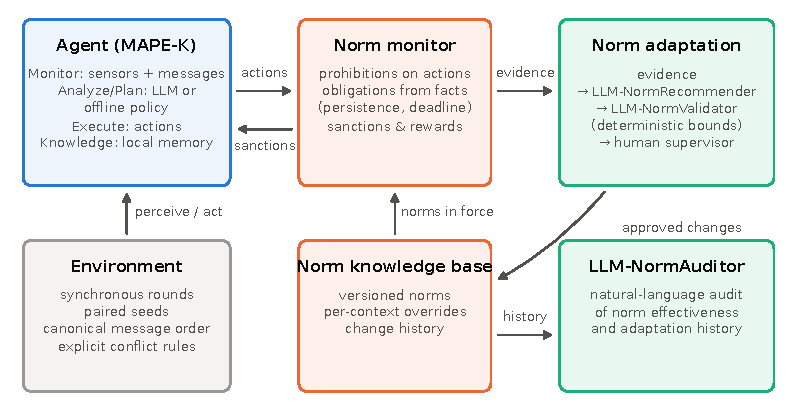
\includegraphics[width=0.92\textwidth]{figures/viana2.pdf}
\caption{Architecture of llm-mas. Every LLM component (agent reasoning, recommender, validator review, auditor) has a deterministic counterpart, so conditions can be compared pairwise on identical environments.}
\label{fig:2}
\end{figure*}

\subsection{Scenarios}\label{sec:3.3}
\begin{table*}[!t]
\centering
\caption{Scenarios, agents, norms and the role played by the LLM.}
\label{tab:1}
\footnotesize
\setlength{\tabcolsep}{0.06cm}
\renewcommand{\arraystretch}{1.15}
\begin{tabular}{@{}>{\raggedright\arraybackslash}p{\dimexpr0.170\textwidth-0.12cm\relax}>{\raggedright\arraybackslash}p{\dimexpr0.200\textwidth-0.12cm\relax}>{\raggedright\arraybackslash}p{\dimexpr0.250\textwidth-0.12cm\relax}>{\raggedright\arraybackslash}p{\dimexpr0.180\textwidth-0.12cm\relax}>{\raggedright\arraybackslash}p{\dimexpr0.200\textwidth-0.12cm\relax}@{}}
\hline
\textbf{Scenario} & \textbf{Agents} & \textbf{Norms} & \textbf{Role of the LLM} & \textbf{Main metrics} \\ \hline
Book marketplace (from \cite{nascimento2023selfadaptive}) & 3 sellers, 2 buyers; 3 iterations & no self-messages; no impersonation; Confirm\_sale only after a matching Buy\_Book & all five agents negotiate in free text & sales, price, unsold sellers, norm violations \\
ICU alarm management (from \cite{viana2025anaml2}) & 2 monitors, 1 alerting agent, 1 decision agent; 12 patients; 120 iterations & 4 adaptable alarm obligations (SpO\textsubscript{2}, HR, SBP, RR) + 1 critical, non-adaptable & norm recommender (RQ2) or decision agent (RQ3) & false alarms, sensitivity, latency, verdict accuracy \\
Project management (dynamic contexts) & 1 manager, 4–5 developers; 60 iterations & WIP limit (prohibition); assign unowned tasks within 2 iterations (obligation) & manager allocates tasks under 5 context events & completion iteration, tasks done, violations \\ \hline
\end{tabular}
\end{table*}

In the ICU scenario, patients belong to four physiological profiles (no chronic disease, COPD, chronic tachycardia, chronic hypotension); half of them develop a 10-iteration deterioration episode, and 5\% of SpO\textsubscript{2} readings are motion artifacts. The alerting agent fulfills alarm obligations; the decision agent judges whether each alarm reflects real deterioration; those verdicts become the evidence on which norms are adapted per patient (e.g., a lower SpO\textsubscript{2} threshold and 2-reading persistence for a COPD patient). The project scenario injects requirement changes, a developer leaving and another joining, a bug spike and a productivity drop.

\subsection{Imperfect evidence, baselines and ceiling}\label{sec:3.4}
A naive ICU simulation can leak the ground truth to the decision agent—for instance, through a bedside report that states ``signs of deterioration'' exactly when the alarm is real. We replaced it with an observation model: bedside findings (dyspnea, sweating, altered consciousness, slow capillary refill, complaint) occur with partial sensitivity and specificity that grow with the deterioration stage, chronic conditions produce baseline findings (e.g., 50\% dyspnea in COPD), and a poor plethysmography signal appears in 70\% of artifacts and 10\% of clean readings. The decision agent receives the triggering reading, the last six readings, the chronic diagnosis and the findings—never the hidden state. True outcomes are confirmed only 30 iterations after an alarm; until then, adaptation relies on the decision agent's verdicts, errors included.

The offline decision policy is a modified NEWS2 score \cite{rcp2017news2}: NEWS2 points on the triggering vital signs (scale 2 for COPD), plus one point per bedside finding, minus two points when an artifact is suspected; an alarm is deemed real when the score is $\geq$ 5, the NEWS2 threshold for urgent review. The threshold was fixed before any run and does not use the generator's parameters. As a ceiling we compute, on the same alarms, a Bayes-optimal classifier that knows the generative model, marginalizing over deterioration stage and artifact occurrence; it is a reference, never a policy.

\subsection{Experimental conditions and controls}\label{sec:3.5}
\begin{table*}[!t]
\centering
\caption{ICU conditions. Each LLM condition differs from adaptive-heuristic in exactly one component.}
\label{tab:2}
\footnotesize
\setlength{\tabcolsep}{0.06cm}
\renewcommand{\arraystretch}{1.15}
\begin{tabular}{@{}>{\raggedright\arraybackslash}p{\dimexpr0.220\textwidth-0.12cm\relax}>{\raggedright\arraybackslash}p{\dimexpr0.200\textwidth-0.12cm\relax}>{\raggedright\arraybackslash}p{\dimexpr0.200\textwidth-0.12cm\relax}>{\raggedright\arraybackslash}p{\dimexpr0.380\textwidth-0.12cm\relax}@{}}
\hline
\textbf{Condition} & \textbf{Norm recommender} & \textbf{Decision agent} & \textbf{Purpose} \\ \hline
static & — & NEWS2 & traditional, non-adaptive baseline \\
adaptive-oracle & deterministic & oracle (true labels) & upper reference for adaptation \\
adaptive-heuristic & deterministic & NEWS2 & non-LLM adaptive baseline ($\Delta$ reference) \\
adaptive-llm & \textbf{LLM} & NEWS2 & RQ2: only the recommender changes \\
adaptive-llm-decision & deterministic & \textbf{LLM} & RQ3: only the decision agent changes \\ \hline
\end{tabular}
\end{table*}

All conditions are paired by seed: the same seed yields the same patients, readings, bedside findings (drawn from a seed derived from patient and iteration) and project scenario. The platform is order-invariant by construction and by test: results do not depend on the order in which agents are registered (Section~\ref{sec:4.4}). Commands such as \texttt{Buy\_Book: 30} or \texttt{assign T3} take effect only when they are the entire message; the environment notifies agents of commands without effect. Prompts state the same protocol rules that the heuristic policies follow by construction.

\subsection{Model, cost and analysis}\label{sec:3.6}
We used Claude Opus 5.5 (\texttt{claude-opus-5-5}) with effort \emph{low}, structured JSON outputs for the recommender and decision agent, and server-side refusal fallback. Before spending, a dry run executed the whole experiment with a recording client and estimated US\$ 4.76 from token counts calibrated on earlier runs and one paid probe; the actual cost was US\$ 4.73 for 272 calls (529,296 input and 130,820 output tokens), with no API failures (Table~\ref{tab:9}). We ran three seeds (0–2) per condition. We report means $\pm$ standard deviations and paired differences; for significance we use the exact two-sided sign-flip permutation test on paired differences. With n = 3, its smallest attainable p-value is 0.25, so no comparison can reach conventional significance: this study is exploratory by design.

\subsection{Study 2: deciding whether to comply}\label{sec:3.7}
Study 2 reuses the ICU scenario with \emph{static} norms and makes the alerting agent deliberative, following the ANA normative process \cite{viana2022creating}: \emph{awareness} of each newly opened alarm obligation, \emph{deliberation}, a \emph{compliance} decision—raise the alarm (comply) or suppress it (violate)—and \emph{impact} on its beliefs when sanctions or outcomes arrive. Each obligation is decided once. The critical norm (SpO\textsubscript{2} $<$ 85\% or equivalent) is \emph{regimented}: the architecture always raises it, so every episode is eventually alarmed and the clinical cost of suppression appears as delay. The other four alarm norms are \emph{regulated}: a violation is detected with probability p and then sanctioned; undetected violations are recorded for analysis only.

The agent's goals carry ANA \emph{Motivation} values—patient safety 10 and avoiding alarm fatigue 6—and suppressing an alarm it judges false has \emph{Satisfaction} 3. Each fulfilled obligation is rewarded with 1 point and each detected violation sanctioned with 5 points times a sanction scale. The outcome of every suppressed alarm is confirmed 30 iterations after the reading; if a real deterioration was suppressed before any true alarm of that episode, a harm penalty of 20 is charged, once per episode. These values were fixed before any run. Offline strategies judge an alarm real when the modified NEWS2 score of Study 1 is $\geq$ 5 (Table~\ref{tab:3}).

\begin{table}[!t]
\centering
\caption{Compliance strategies, operationalized from \cite{lopez2002constraining} on the same information given to the LLM.}
\label{tab:3}
\footnotesize
\setlength{\tabcolsep}{0.06cm}
\renewcommand{\arraystretch}{1.15}
\begin{tabular}{@{}>{\raggedright\arraybackslash}p{\dimexpr0.180\columnwidth-0.12cm\relax}>{\raggedright\arraybackslash}p{\dimexpr0.820\columnwidth-0.12cm\relax}@{}}
\hline
\textbf{Strategy} & \textbf{Decision rule (operationalization)} \\ \hline
social & always complies \\
rebellious & violates whenever the architecture allows (any non-regimented obligation) \\
selfish & violates when violating favors its own goals (it judges the alarm false), ignoring sanctions \\
pressured & violates only if the gain of violating exceeds detection $\times$ sanction + reward \\
opportunistic & violates when it favors its goals and detection is unlikely (p $<$ 0.5) \\
LLM & decides in natural language from the same information, returning belief, decision and justification \\ \hline
\end{tabular}
\end{table}

The LLM deliberative agent receives, for each pending obligation, the same evidence as the decision agent of Study 1 (triggering reading, six-reading trend, chronic diagnosis, bedside findings), the reward, sanction and detection probability, its goals, and a permanent normative record (obligations fulfilled, sanctions, confirmed outcomes of past suppressions, harms). It returns, per patient, whether it believes the deterioration is real, whether it complies, and why. A failed or missing answer defaults to compliance and is counted; runs with more than 5\% defaulted decisions are excluded. As in Study 1, all prompts are written in Portuguese and the model answers through a JSON schema whose patient field is restricted to the pending obligations.

The agent instantiates the ANA-BDI loop (Fig.~\ref{fig:1}): the norm monitor \emph{collects} each new alarm obligation; a deliberation strategy \emph{analyzes} it; the \emph{decision} is to comply or violate; and the \emph{effector} raises or suppresses the alarm. In JSAN, deliberation is a framework hot spot, \texttt{NormDeliberation}, plugged into the frozen \texttt{Analyze} behavior through the \texttt{IReasoningStrategy} interface (Fig.~\ref{fig:3}). Our five classical strategies and the LLM are interchangeable implementations of this one hot spot: they receive the same case—norms, reward, sanction, detection probability and the evidence—and return a decision. The comparison therefore isolates the reasoning strategy, which is exactly the variation point that ANA-ML 2.0 proposes to fill with an LLM. Its operations map onto our deliberation case as follows: \emph{conditionNorms} selects the regulated (non-regimented) obligations; \emph{fulfillingNorms} weighs the reward of compliance; \emph{normativeContribution} weighs the expected sanction and the risk of harm against the goal of avoiding alarm fatigue; and \emph{detectingSolvingConflicts} resolves the conflict between the agent's two goals.

\begin{figure*}[!t]
\centering
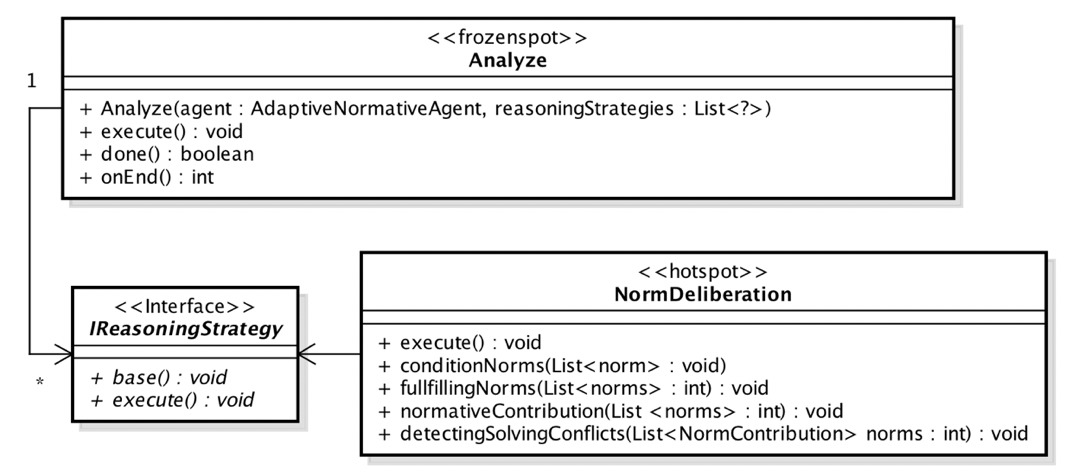
\includegraphics[width=0.95\textwidth]{figures/viana3.png}
\caption{Norm deliberation as a hot spot of the JSAN framework \cite{viana2015jsan}. The classical strategies and the LLM of Study 2 are alternative implementations of this hot spot.}
\label{fig:3}
\end{figure*}

\begin{table*}[!t]
\centering
\caption{Study 2 conditions (3 paired seeds each).}
\label{tab:4}
\footnotesize
\setlength{\tabcolsep}{0.06cm}
\renewcommand{\arraystretch}{1.15}
\begin{tabular}{@{}>{\raggedright\arraybackslash}p{\dimexpr0.200\textwidth-0.12cm\relax}>{\raggedright\arraybackslash}p{\dimexpr0.180\textwidth-0.12cm\relax}>{\raggedright\arraybackslash}p{\dimexpr0.240\textwidth-0.12cm\relax}>{\raggedright\arraybackslash}p{\dimexpr0.180\textwidth-0.12cm\relax}>{\raggedright\arraybackslash}p{\dimexpr0.200\textwidth-0.12cm\relax}@{}}
\hline
\textbf{Condition} & \textbf{Norms} & \textbf{Compliance} & \textbf{Detection p} & \textbf{Sanction scale} \\ \hline
adaptive-compliant & adaptive (Study 1) & always & — & — \\
strategies & static & 5 strategies (Table~\ref{tab:3}) & 0.3, 0.7, 1.0 & 0.2, 1, 3 \\
LLM & static & LLM deliberation & 0.3, 0.7, 1.0 & 1 \\ \hline
\end{tabular}
\end{table*}

\textbf{Metrics.} Besides false alarms and latency, we report suppressions, split into \emph{justified} (the alarm was false) and \emph{of real deterioration}; \emph{harmed episodes}, in which a suppression delayed recognition; violations, all and detected; \emph{social contribution}, the share of obligations on real deterioration that were complied with; and the agent's \emph{individual satisfaction}—action satisfaction plus rewards minus detected sanctions and harm penalties \cite{viana2015jsan}. For the LLM we also report belief accuracy and decision–belief coherence.

\textbf{Verification before spending.} Because the LLM runs are costly, the environment was verified first: (i) all 15 offline Study 1 runs were reproduced exactly after the Study 2 changes; (ii) 13 equivalence tests replace the LLM with an emulator that reads only the prompt text and applies an offline rule—the simulations are identical to those of the corresponding offline policy for all five strategies, two detection levels and a different sanction scale, and for the Study 1 decision agent and recommender—showing that prompts carry the information the policies use and that answers are parsed and applied correctly; (iii) ten invariant tests cover determinism, pairing, order invariance and metric accounting; (iv) a second independent code review found four defects, fixed before any paid run (Table~\ref{tab:8}, rows 10–14); and (v) the output schema was validated against the API at no cost. A dry run estimated 930 calls (about US\$ 15.35) for the LLM conditions.

\textbf{Execution.} The nine LLM runs (three seeds $\times$ three detection levels) made 930 valid calls, as estimated, but the dry run underestimated the length of the justifications (524,263 output tokens in total against 338,400 estimated). The budget cap therefore stopped the planned execution during its last run; that run was discarded, and the missing combination (seed 2, p = 1.0) was executed separately with the same code. Because the offline strategies are deterministic, we checked that all of their runs were identical across the two executions and the offline study. The total cost was US\$ 17.84 for 948 calls (1,839,420 input and 524,263 output tokens), of which US\$ 0.29 belonged to the discarded run. No call failed and no decision was defaulted.

\textbf{Replay.} Every LLM call is stored with its prompt and answer. For the analysis of RQ7 we re-ran each LLM run offline, answering each prompt with the recorded answer. All nine replays reproduced the recorded metrics exactly, which confirms that the runs are reproducible from their transcripts and gives us, at no cost, the ground truth behind every decision.

\section{Results}\label{sec:4}
\subsection{RQ1 – Negotiation and coordination}\label{sec:4.1}
\begin{table*}[!t]
\centering
\caption{Marketplace and project results (3 paired seeds; mean $\pm$ s.d.; p from exact sign-flip test, minimum 0.25).}
\label{tab:5}
\footnotesize
\setlength{\tabcolsep}{0.06cm}
\renewcommand{\arraystretch}{1.15}
\begin{tabular}{@{}>{\raggedright\arraybackslash}p{\dimexpr0.340\textwidth-0.12cm\relax}>{\raggedright\arraybackslash}p{\dimexpr0.160\textwidth-0.12cm\relax}>{\raggedright\arraybackslash}p{\dimexpr0.160\textwidth-0.12cm\relax}>{\raggedright\arraybackslash}p{\dimexpr0.200\textwidth-0.12cm\relax}>{\raggedright\arraybackslash}p{\dimexpr0.140\textwidth-0.12cm\relax}@{}}
\hline
\textbf{Metric} & \textbf{Heuristic} & \textbf{LLM} & \textbf{$\Delta$ (LLM $-$ heur.)} & \textbf{p} \\ \hline
Sales per run & 1.0 $\pm$ 0.0 & 2.0 $\pm$ 0.0 & 1.0 $\pm$ 0.0 & 0.25 \\
Mean sale price (US\$) & 21.0 $\pm$ 1.0 & 31.7 $\pm$ 1.4 & 10.7 $\pm$ 1.8 & 0.25 \\
Buyers without a book & 1.0 $\pm$ 0.0 & 0.0 $\pm$ 0.0 & -1.0 $\pm$ 0.0 & 0.25 \\
Messages & 27.0 $\pm$ 0.0 & 37.7 $\pm$ 1.5 & 10.7 $\pm$ 1.5 & 0.25 \\
Self-messages & 0 $\pm$ 0 & 0 $\pm$ 0 & 0 & — \\
Norm violations (total, 3 runs) & 0 & 1 &  &  \\
\textbf{Project:} completion iteration & 33.0 $\pm$ 2.6 & 35.0 $\pm$ 1.0 & 2.0 $\pm$ 2.0 & 0.50 \\
\textbf{Project:} tasks completed & 25 $\pm$ 0 & 25 $\pm$ 0 & 0 & — \\
\textbf{Project:} backlog-norm violations & 0 & 0 &  &  \\ \hline
\end{tabular}
\end{table*}

LLM agents completed two sales in every run (vs. one), leaving no buyer without a book, and sold at higher prices (US\$ 31.7 vs. 21.0). Initial asking prices varied widely (US\$ 8–50): some sellers anchored high and conceded, others undercut aggressively; buyers broadcast offers to several sellers; the explicit conflict rule (earliest matching order wins) resolved simultaneous confirmations. No agent sent messages to itself. The single violation was genuine rather than a simulator artifact: a seller sent two confirmations at different prices to the same buyer, one of which no longer matched the buyer's order. The heuristic baseline is weak in this scenario—both heuristic buyers always target the cheapest seller—so the size of the LLM advantage should not be generalized.

In project management, both managers completed all tasks without backlog-norm violations; the LLM manager finished 2.0 iterations later on average (p = 0.50). The only violations were WIP-limit breaches by a developer configured as undisciplined, identical in both conditions, after which the developer adapted to the sanction. \textbf{Answer to RQ1:} LLM agents negotiated more effectively and respected the protocol norms; in task allocation, they matched but did not surpass a load-balancing heuristic.

\subsection{RQ2 – LLM-based norm recommendation}\label{sec:4.2}
\begin{figure*}[!t]
\centering
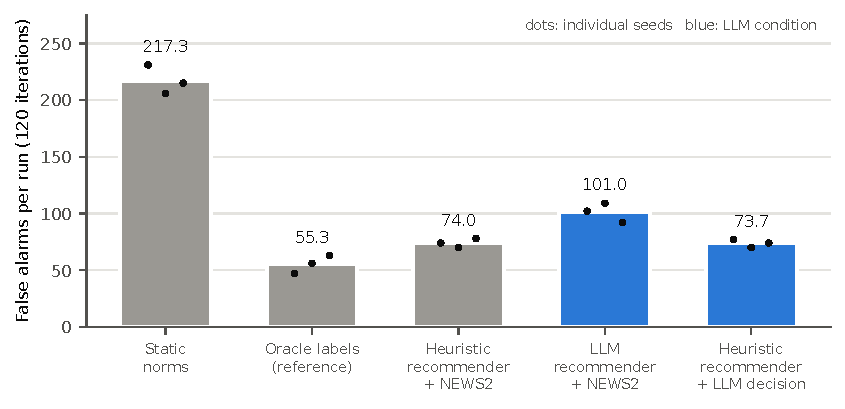
\includegraphics[width=0.92\textwidth]{figures/viana4.pdf}
\caption{ICU false alarms per run by condition (bars: mean of 3 seeds; dots: seeds). Blue bars change exactly one component to an LLM relative to the heuristic condition.}
\label{fig:4}
\end{figure*}

\begin{table*}[!t]
\centering
\caption{ICU results by condition (3 paired seeds, mean $\pm$ s.d.). LLM rec. = adaptive-llm; LLM dec. = adaptive-llm-decision. No norm violations and no LLM failures occurred in any condition.}
\label{tab:6}
\footnotesize
\setlength{\tabcolsep}{0.06cm}
\renewcommand{\arraystretch}{1.15}
\begin{tabular}{@{}>{\raggedright\arraybackslash}p{\dimexpr0.300\textwidth-0.12cm\relax}>{\raggedright\arraybackslash}p{\dimexpr0.140\textwidth-0.12cm\relax}>{\raggedright\arraybackslash}p{\dimexpr0.140\textwidth-0.12cm\relax}>{\raggedright\arraybackslash}p{\dimexpr0.140\textwidth-0.12cm\relax}>{\raggedright\arraybackslash}p{\dimexpr0.140\textwidth-0.12cm\relax}>{\raggedright\arraybackslash}p{\dimexpr0.140\textwidth-0.12cm\relax}@{}}
\hline
\textbf{Metric} & \textbf{Static} & \textbf{Oracle} & \textbf{Heuristic} & \textbf{LLM rec.} & \textbf{LLM dec.} \\ \hline
False alarms & 217.3 $\pm$ 12.7 & 55.3 $\pm$ 8.0 & 74.0 $\pm$ 4.0 & 101.0 $\pm$ 8.5 & 73.7 $\pm$ 3.5 \\
Sensitivity (alarm raised) & 1.00 $\pm$ 0.00 & 1.00 $\pm$ 0.00 & 1.00 $\pm$ 0.00 & 1.00 $\pm$ 0.00 & 1.00 $\pm$ 0.00 \\
Specificity & 0.843 $\pm$ 0.008 & 0.960 $\pm$ 0.006 & 0.947 $\pm$ 0.003 & 0.927 $\pm$ 0.007 & 0.947 $\pm$ 0.002 \\
Alarm latency (it.) & 1.79 $\pm$ 0.22 & 2.16 $\pm$ 0.91 & 2.16 $\pm$ 0.91 & 1.79 $\pm$ 0.54 & 2.16 $\pm$ 0.91 \\
Episodes recognized & 1.00 $\pm$ 0.00 & 1.00 $\pm$ 0.00 & 1.00 $\pm$ 0.00 & 1.00 $\pm$ 0.00 & 1.00 $\pm$ 0.00 \\
Recognition latency (it.) & 1.79 $\pm$ 0.22 & 2.16 $\pm$ 0.91 & 2.16 $\pm$ 0.91 & 1.79 $\pm$ 0.54 & 2.50 $\pm$ 0.44 \\
Norm changes applied & 0.0 $\pm$ 0.0 & 17.3 $\pm$ 0.6 & 16.3 $\pm$ 1.2 & 12.7 $\pm$ 3.1 & 16.3 $\pm$ 1.2 \\
Wrong labels used in reviews & 0.0 $\pm$ 0.0 & 0.0 $\pm$ 0.0 & 34.3 $\pm$ 7.6 & 38.7 $\pm$ 7.6 & 33.3 $\pm$ 2.5 \\
Verdict accuracy & 0.822 $\pm$ 0.018 & 1.000 $\pm$ 0.000 & 0.802 $\pm$ 0.024 & 0.801 $\pm$ 0.005 & 0.815 $\pm$ 0.001 \\
Verdict sensitivity & 1.00 $\pm$ 0.00 & 1.00 $\pm$ 0.00 & 1.00 $\pm$ 0.00 & 1.00 $\pm$ 0.00 & 0.96 $\pm$ 0.08 \\
Verdict specificity & 0.801 $\pm$ 0.023 & 1.000 $\pm$ 0.000 & 0.735 $\pm$ 0.028 & 0.750 $\pm$ 0.010 & 0.764 $\pm$ 0.029 \\
Bayes-optimal accuracy (same alarms) & 0.991 $\pm$ 0.009 & 0.979 $\pm$ 0.008 & 0.983 $\pm$ 0.006 & 0.984 $\pm$ 0.009 & 0.987 $\pm$ 0.006 \\ \hline
\end{tabular}
\end{table*}

Adaptation was effective: relative to static norms, the deterministic recommender reduced false alarms by 66\% (217.3 $\rightarrow$ 74.0) and perfect labels would reduce them by 75\%, with sensitivity preserved at 1.0 in every condition and the critical norm never altered. A five-seed offline replication confirmed the effect (210.2 $\rightarrow$ 69.4; paired t = 30.48, df = 4). The LLM recommender, however, was worse than the deterministic one: 101.0 vs. 74.0 false alarms ($\Delta$ = 27.0 $\pm$ 12.5, worse in all three seeds, p = 0.25). It applied fewer changes (12.7 vs. 16.3), and 15 of its 21 responses mentioned that verdicts were not yet confirmed by outcomes. In one seed, the LLM-NormAuditor's report likewise noted that adaptations relied largely on unconfirmed verdicts and recommended suspending further adaptation until confirmation—a cautious stance that, here, left avoidable false alarms in place.

\begin{figure}[!t]
\centering
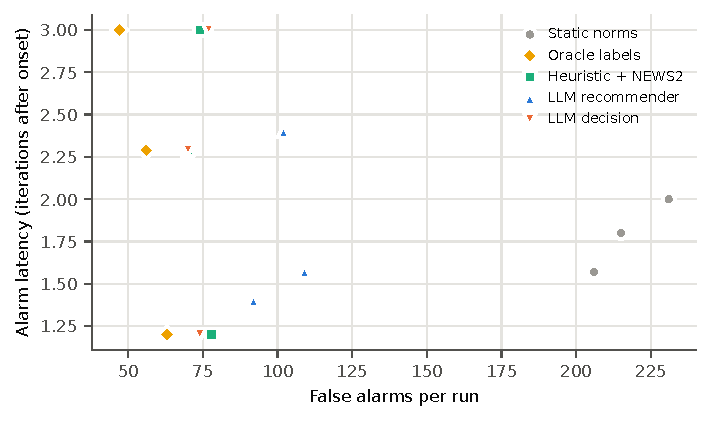
\includegraphics[width=\columnwidth]{figures/viana5.pdf}
\caption{False alarms versus alarm latency per seed. Adaptation moves runs to the left (fewer false alarms) but tends to move them up (later alarms); the LLM recommender adapts less and sits between static and heuristic adaptation.}
\label{fig:5}
\end{figure}

The flip side is latency (Fig.~\ref{fig:5}). Adaptation raised mean alarm latency from 1.79 to 2.16 iterations (in the offline replication, from 1.50 to 2.03, higher in 4 of 5 seeds), because per-patient thresholds and 2-reading persistence delay the first alarm of an episode; the LLM recommender's latency (1.79) stayed at the static level precisely because it adapted less. \textbf{Answer to RQ2:} adaptive norms reduced false alarms substantially without missing episodes, but the LLM recommender did not improve on a deterministic recommender and adapted more conservatively; neither reduced response time.

\subsection{RQ3 – LLM decision under imperfect evidence}\label{sec:4.3}
\begin{figure}[!t]
\centering
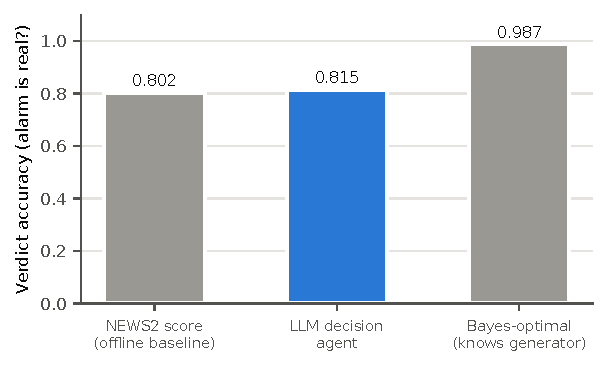
\includegraphics[width=\columnwidth]{figures/viana6.pdf}
\caption{Accuracy of alarm verdicts (is the alarm real?). The Bayes-optimal classifier knows the generative model and serves only as a ceiling.}
\label{fig:6}
\end{figure}

\begin{table*}[!t]
\centering
\caption{Verdicts of the LLM decision agent per patient profile, reconstructed from the transcripts against the simulator's ground truth.}
\label{tab:7}
\footnotesize
\setlength{\tabcolsep}{0.06cm}
\renewcommand{\arraystretch}{1.15}
\begin{tabular}{@{}>{\raggedright\arraybackslash}p{\dimexpr0.280\textwidth-0.12cm\relax}>{\raggedright\arraybackslash}p{\dimexpr0.120\textwidth-0.12cm\relax}>{\raggedright\arraybackslash}p{\dimexpr0.120\textwidth-0.12cm\relax}>{\raggedright\arraybackslash}p{\dimexpr0.170\textwidth-0.12cm\relax}>{\raggedright\arraybackslash}p{\dimexpr0.170\textwidth-0.12cm\relax}>{\raggedright\arraybackslash}p{\dimexpr0.140\textwidth-0.12cm\relax}@{}}
\hline
\textbf{Patient profile} & \textbf{Alarms} & \textbf{Real} & \textbf{False positives} & \textbf{False negatives} & \textbf{Accuracy} \\ \hline
No chronic disease & 42 & 11 & 10 & 0 & 0.762 \\
COPD & 73 & 15 & 9 & 0 & 0.877 \\
Chronic tachycardia & 96 & 33 & 16 & 2 & 0.812 \\
Chronic hypotension & 86 & 17 & 17 & 1 & 0.791 \\
All & 297 & 76 & 52 & 3 & 0.815 \\ \hline
\end{tabular}
\end{table*}

The LLM decision agent reached an accuracy of 0.815, against 0.802 for the NEWS2 policy (paired $\Delta$ = 0.013 $\pm$ 0.023, p = 0.50) and 0.987 for the Bayes ceiling. It traded a little sensitivity (0.96 vs. 1.00) for specificity (0.764 vs. 0.735), with no net effect on false alarms (73.7 vs. 74.0), and recognized episodes slightly later (2.50 vs. 2.16 iterations). Of its 297 verdicts, 52 were false positives and 3 false negatives (Table~\ref{tab:7}). Inspection of the errors shows that most false positives occurred when the evidence genuinely looked concerning—spurious findings or artifacts without a visible signal problem—and that the justifications were clinically coherent (e.g., attributing a systolic pressure of 88 mmHg to chronic hypotension). The gap to the ceiling reflects knowledge that no clinician has—the exact noise distributions—rather than a failure of reasoning. \textbf{Answer to RQ3:} under imperfect evidence, the LLM decision agent performed on par with an established clinical score, with interpretable justifications but no accuracy gain.

\subsection{RQ4 – Engineering threats to validity}\label{sec:4.4}
Table~\ref{tab:8} lists the problems found while building the study, how each was detected, what it would have done to the results, and the control adopted. Detection came from four sources: our own measurements, inspection of LLM transcripts, an independent automated code review performed by a separate LLM agent with no access to our reasoning, and—notably—the LLM-NormAuditor, whose report on an early run pointed out that alarms were recorded with vital signs that satisfied none of their norms.

\begin{table*}[!t]
\centering
\caption{Engineering threats to validity found while building the study, with their detection source, potential effect and control.}
\label{tab:8}
\footnotesize
\setlength{\tabcolsep}{0.06cm}
\renewcommand{\arraystretch}{1.15}
\begin{tabular}{@{}>{\raggedright\arraybackslash}p{\dimexpr0.040\textwidth-0.12cm\relax}>{\raggedright\arraybackslash}p{\dimexpr0.240\textwidth-0.12cm\relax}>{\raggedright\arraybackslash}p{\dimexpr0.150\textwidth-0.12cm\relax}>{\raggedright\arraybackslash}p{\dimexpr0.300\textwidth-0.12cm\relax}>{\raggedright\arraybackslash}p{\dimexpr0.270\textwidth-0.12cm\relax}@{}}
\hline
\textbf{\#} & \textbf{Threat} & \textbf{Detected by} & \textbf{Effect if unnoticed} & \textbf{Control} \\ \hline
1 & Execution-order bias via mid-round state, mailbox order and a shared RNG & measurement (agent permutations) & 97\% of marketplace outcomes changed with agent order; first-acting seller made 67\% of sales (expected 33\%) & synchronous rounds; seeded canonical mailbox order; per-agent RNG; explicit conflict rule \\
2 & Alarm stored the reading of the alarm iteration, not the triggering one & LLM-NormAuditor & 62\% of alarms carried vitals that triggered none of their norms; adaptation fed with wrong evidence & store the triggering reading per norm \\
3 & Ground truth, latency and specificity judged at alarm time (one iteration late) & independent code review & latency increase overstated about 2$\times$; boundary alarms mislabeled & judge by reading iteration \\
4 & Bedside report leaked the ground truth & design review & decision reduced to keyword lookup & stochastic findings; NEWS2 baseline; Bayes ceiling \\
5 & Commands detected anywhere in free text & LLM transcripts & a refusal quoting ``Confirm\_sale: 30'' counted as a confirmation and was sanctioned & commands valid only as the whole message; environment feedback \\
6 & Obligation fulfilled by an ineffective action; latch hid neglect & independent code review & a manager assigning all tasks to a departed developer: 0 tasks done, 0 violations & count only effective assignments; re-arm obligations \\
7 & Prompt and code disagreed on the meaning of persistence = 1 & independent code review & following the prompt silently removed 2-reading persistence in LLM runs only & 0 = keep current, in prompt and code \\
8 & Unpaired aggregation; fatal errors & independent code review & failed seeds dropped from one column only; an unknown task id aborted all paid runs & paired tables; censoring; per-run fault tolerance \\
9 & Uncontrolled cost & dry run & — & dry-run estimate (US\$ 4.76) vs. actual (US\$ 4.73); budget cap; skip calls for agents with nothing to decide \\
10 & \textbf{Study 2:} failed LLM calls defaulted silently to compliance & independent code review & a run in which every call failed was indistinguishable from the social strategy & defaulted decisions counted; runs above 5\% excluded and listed \\
11 & A suppressed obligation fulfilled by an alarm for another norm of the same patient & independent code review & suppression rewarded as fulfillment, violation never recorded (2–3 per run) & an alarm fulfills only the norms it declares \\
12 & Harm counted per suppressed obligation & independent code review & up to three penalties per episode, also when the episode had already been alarmed & one harm per episode, only if the suppression delayed recognition \\
13 & Bounded working memory evicted old sanctions & independent code review & prompt section ``sanctions received'' omitted most of them & permanent normative record \\
14 & Detection draws not paired across conditions & independent code review & the same violation detected in one condition and not in another & per-violation seeded draw \\
15 & Sanction history in the prompt listed rewards & prompt inspection & misleading feedback to the LLM & only sanctions, harms and confirmed outcomes shown \\
16 & Pressured and opportunistic strategies indistinguishable & offline pilot & two strategies collapsed at a single sanction level & sanction size added as a factor \\
17 & Dry run underestimated the length of LLM justifications & budget cap during the paid run & execution stopped in its last run; US\$ 0.29 of calls discarded & results saved per run; missing run executed separately; offline runs checked identical; replay of transcripts reproduces every metric \\ \hline
\end{tabular}
\end{table*}

\begin{figure}[!t]
\centering
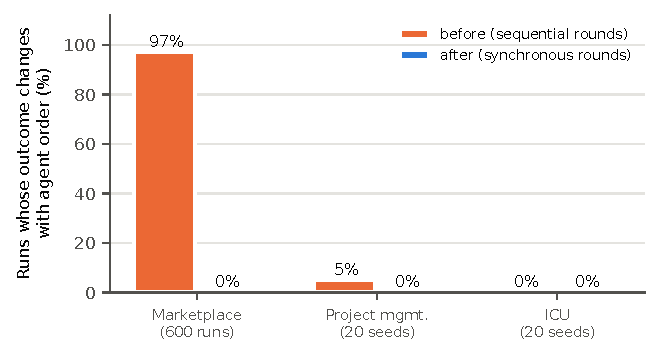
\includegraphics[width=\columnwidth]{figures/viana7.pdf}
\caption{Share of runs whose outcome changes when the agent registration order is permuted, before and after introducing synchronous rounds (offline policies; marketplace: 50 seeds $\times$ 12 orders).}
\label{fig:7}
\end{figure}

\begin{table*}[!t]
\centering
\caption{Cost of the LLM runs by component and study (Claude Opus 5.5, effort low, US\$ 4/20 per million input/output tokens).}
\label{tab:9}
\footnotesize
\setlength{\tabcolsep}{0.06cm}
\renewcommand{\arraystretch}{1.15}
\begin{tabular}{@{}>{\raggedright\arraybackslash}p{\dimexpr0.360\textwidth-0.12cm\relax}>{\raggedright\arraybackslash}p{\dimexpr0.100\textwidth-0.12cm\relax}>{\raggedright\arraybackslash}p{\dimexpr0.180\textwidth-0.12cm\relax}>{\raggedright\arraybackslash}p{\dimexpr0.180\textwidth-0.12cm\relax}>{\raggedright\arraybackslash}p{\dimexpr0.180\textwidth-0.12cm\relax}@{}}
\hline
\textbf{Component} & \textbf{Calls} & \textbf{Input tokens} & \textbf{Output tokens} & \textbf{Cost (US\$)} \\ \hline
ICU decision agent & 199 & 232,646 & 76,086 & 2.45 \\
ICU LLM-NormRecommender & 21 & 219,034 & 21,143 & 1.30 \\
Marketplace agents & 37 & 44,709 & 15,130 & 0.48 \\
Project manager agent & 12 & 21,380 & 9,974 & 0.28 \\
ICU LLM-NormAuditor & 3 & 11,527 & 8,487 & 0.22 \\
Total, Study 1 & 272 & 529,296 & 130,820 & 4.73 \\
Study 2: LLM deliberation (incl. discarded run) & 948 & 1,839,420 & 524,263 & 17.84 \\ \hline
\end{tabular}
\end{table*}

\textbf{Answer to RQ4:} threats 1–8 could each have produced a spurious difference between conditions or a distorted metric—several of them of the same order as the effects we measured—and threat 9 could have made the study unaffordable to replicate. Threats 10–16 of Study 2 were all found and fixed before any paid run; threat 17 affected only cost and was contained by per-run persistence. Synchronous rounds, pairing by seed, one-variable-at-a-time conditions, information parity in prompts, explicit protocol semantics, and transcript-level auditing were all necessary to obtain a fair comparison.

\section{Results of Study 2}\label{sec:5}
\subsection{RQ5 – Deviating from norms versus adapting them}\label{sec:5.1}
\begin{table*}[!t]
\centering
\caption{Study 2 at detection p = 0.3 and default sanction (3 paired seeds, mean $\pm$ s.d.). ``Of real deterior.'' counts suppressed obligations during a real deterioration; ``harmed episodes'' counts episodes whose recognition a suppression delayed.}
\label{tab:10}
\footnotesize
\setlength{\tabcolsep}{0.06cm}
\renewcommand{\arraystretch}{1.15}
\begin{tabular}{@{}>{\raggedright\arraybackslash}p{\dimexpr0.170\textwidth-0.12cm\relax}>{\raggedright\arraybackslash}p{\dimexpr0.100\textwidth-0.12cm\relax}>{\raggedright\arraybackslash}p{\dimexpr0.100\textwidth-0.12cm\relax}>{\raggedright\arraybackslash}p{\dimexpr0.100\textwidth-0.12cm\relax}>{\raggedright\arraybackslash}p{\dimexpr0.100\textwidth-0.12cm\relax}>{\raggedright\arraybackslash}p{\dimexpr0.090\textwidth-0.12cm\relax}>{\raggedright\arraybackslash}p{\dimexpr0.090\textwidth-0.12cm\relax}>{\raggedright\arraybackslash}p{\dimexpr0.100\textwidth-0.12cm\relax}>{\raggedright\arraybackslash}p{\dimexpr0.150\textwidth-0.12cm\relax}@{}}
\hline
\textbf{Condition (p = 0.3)} & \textbf{False alarms} & \textbf{Suppressions} & \textbf{Of real deterior.} & \textbf{Harmed episodes} & \textbf{Alarm latency} & \textbf{Recogn. latency} & \textbf{Social contrib.} & \textbf{Indiv. satisf.} \\ \hline
Comply (social) & 217.3 $\pm$ 12.7 & 0.0 $\pm$ 0.0 & 0.0 $\pm$ 0.0 & 0.0 $\pm$ 0.0 & 1.79 $\pm$ 0.22 & 1.79 $\pm$ 0.22 & 1.000 $\pm$ 0.000 & 254.3 $\pm$ 12.7 \\
Adapt norms (Study 1) & 74.0 $\pm$ 4.0 & 0.0 $\pm$ 0.0 & 0.0 $\pm$ 0.0 & 0.0 $\pm$ 0.0 & 2.16 $\pm$ 0.91 & 2.16 $\pm$ 0.91 & — & 109.7 $\pm$ 0.6 \\
Selfish & 42.7 $\pm$ 3.5 & 174.7 $\pm$ 14.0 & 0.0 $\pm$ 0.0 & 0.0 $\pm$ 0.0 & 1.79 $\pm$ 0.22 & 1.79 $\pm$ 0.22 & 1.000 $\pm$ 0.000 & 347.7 $\pm$ 44.8 \\
Pressured & 43.7 $\pm$ 4.5 & 173.7 $\pm$ 14.6 & 0.0 $\pm$ 0.0 & 0.0 $\pm$ 0.0 & 1.79 $\pm$ 0.22 & 1.79 $\pm$ 0.22 & 1.000 $\pm$ 0.000 & 348.3 $\pm$ 42.8 \\
Opportunistic & 42.7 $\pm$ 3.5 & 174.7 $\pm$ 14.0 & 0.0 $\pm$ 0.0 & 0.0 $\pm$ 0.0 & 1.79 $\pm$ 0.22 & 1.79 $\pm$ 0.22 & 1.000 $\pm$ 0.000 & 347.7 $\pm$ 44.8 \\
Rebellious & 0.0 $\pm$ 0.0 & 235.0 $\pm$ 14.2 & 17.7 $\pm$ 2.5 & 4.0 $\pm$ 1.0 & 4.38 $\pm$ 1.61 & 4.38 $\pm$ 1.61 & 0.000 $\pm$ 0.000 & 129.0 $\pm$ 51.1 \\
\textbf{LLM} & 163.7 $\pm$ 3.1 & 53.7 $\pm$ 12.5 & 0.0 $\pm$ 0.0 & 0.0 $\pm$ 0.0 & 1.79 $\pm$ 0.22 & 1.79 $\pm$ 0.22 & 1.000 $\pm$ 0.000 & 273.0 $\pm$ 31.3 \\ \hline
\end{tabular}
\end{table*}

\begin{figure*}[!t]
\centering
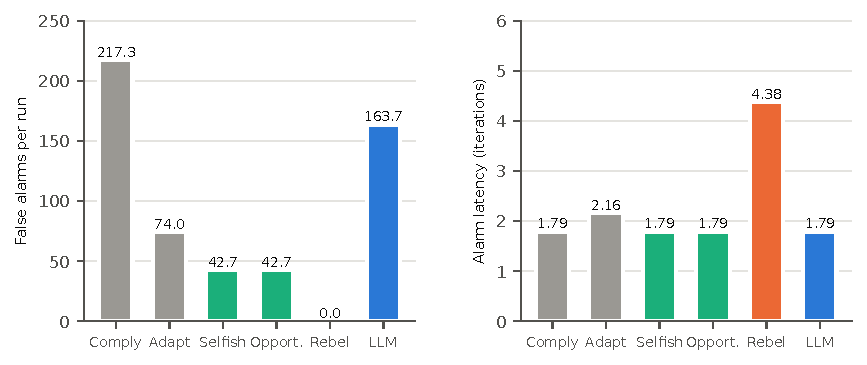
\includegraphics[width=0.95\textwidth]{figures/viana8.pdf}
\caption{False alarms and alarm latency when norms are kept and complied with (Comply), adapted (Adapt, Study 1), or deviated from by an autonomous agent—selfish, opportunistic (Opport.), rebellious (Rebel) or LLM—at p = 0.3.}
\label{fig:8}
\end{figure*}

Keeping static norms and complying produced 217.3 false alarms per run. Adapting the norms (Study 1) reduced them to 74.0 at the cost of a longer latency (2.16 vs. 1.79 iterations). Deviation by a well-informed agent did better on both counts: the selfish strategy left 42.7 false alarms, suppressed 0.0 obligations on real deterioration, harmed 0.0 episodes and kept latency at 1.79. This result hinges on the quality of the agent's belief: the NEWS2-based belief never judged a real deterioration false in this scenario. Uninformed deviation shows the other side—the rebellious agent suppressed every regulated alarm, including 17.7 obligations on real deterioration, harmed 4.0 episodes per run and raised latency to 4.38 iterations; no episode was missed only because the critical norm is regimented. At p = 0.3, rebellion did not pay for the agent itself: its individual satisfaction was 129.0, against 254.3 for the social agent and 347.7 for the selfish one, while its social contribution was 0.00 —harm penalties and lost rewards outweighed the satisfaction of avoided alarms.

The LLM deliberative agent sits between compliance and well-informed deviation (Fig.~\ref{fig:8}). At p = 0.3 it left 163.7 false alarms per run—25\% fewer than compliance, but 121.0 more than the selfish agent and 89.7 more than norm adaptation. It suppressed no obligation on real deterioration, harmed no episode, kept the latency of compliance (1.79 iterations) and a social contribution of 1.00, and obtained an individual satisfaction of 273.0—above the social agent (254.3) and below the selfish one (347.7). Its smaller effect has two sources, which Section~\ref{sec:5.3} examines. First, its beliefs were more cautious than the clinical score: it judged real 34\% of the false alarms at p = 0.3, whereas the NEWS2-based belief judged real 20\%. Second, even when it judged an alarm false it usually complied: it violated only 37\% of the obligations it believed false. \textbf{Answer to RQ5:} deviation can substitute adaptation when the deviating agent's beliefs are accurate, and the regimented safety norm bounds the cost when they are not. The LLM deviated safely but conservatively: it reduced alarm fatigue by about a quarter without any clinical cost, which is less than norm adaptation or a score-guided selfish agent achieved.

\subsection{RQ6 – Enforcement}\label{sec:5.2}
\begin{table*}[!t]
\centering
\caption{Suppressions per run by strategy, detection probability and sanction scale (offline strategies: all scales; LLM: default scale).}
\label{tab:11}
\footnotesize
\setlength{\tabcolsep}{0.06cm}
\renewcommand{\arraystretch}{1.15}
\begin{tabular}{@{}>{\raggedright\arraybackslash}p{\dimexpr0.200\textwidth-0.12cm\relax}>{\raggedright\arraybackslash}p{\dimexpr0.140\textwidth-0.12cm\relax}>{\raggedright\arraybackslash}p{\dimexpr0.220\textwidth-0.12cm\relax}>{\raggedright\arraybackslash}p{\dimexpr0.220\textwidth-0.12cm\relax}>{\raggedright\arraybackslash}p{\dimexpr0.220\textwidth-0.12cm\relax}@{}}
\hline
\textbf{Strategy} & \textbf{Sanction $\times$} & \textbf{p = 0.3} & \textbf{p = 0.7} & \textbf{p = 1} \\ \hline
selfish & 0.2 & 175 $\pm$ 14 & 175 $\pm$ 14 & 175 $\pm$ 14 \\
selfish & 1 & 175 $\pm$ 14 & 175 $\pm$ 14 & 175 $\pm$ 14 \\
selfish & 3 & 175 $\pm$ 14 & 175 $\pm$ 14 & 175 $\pm$ 14 \\
pressured & 0.2 & 175 $\pm$ 14 & 174 $\pm$ 15 & 174 $\pm$ 15 \\
pressured & 1 & 174 $\pm$ 15 & 0 $\pm$ 0 & 0 $\pm$ 0 \\
pressured & 3 & 0 $\pm$ 0 & 0 $\pm$ 0 & 0 $\pm$ 0 \\
opportunistic & 0.2 & 175 $\pm$ 14 & 0 $\pm$ 0 & 0 $\pm$ 0 \\
opportunistic & 1 & 175 $\pm$ 14 & 0 $\pm$ 0 & 0 $\pm$ 0 \\
opportunistic & 3 & 175 $\pm$ 14 & 0 $\pm$ 0 & 0 $\pm$ 0 \\
\textbf{LLM} & 1 & 54 $\pm$ 13 & 3 $\pm$ 4 & 1 $\pm$ 1 \\ \hline
\end{tabular}
\end{table*}

\begin{figure}[!t]
\centering
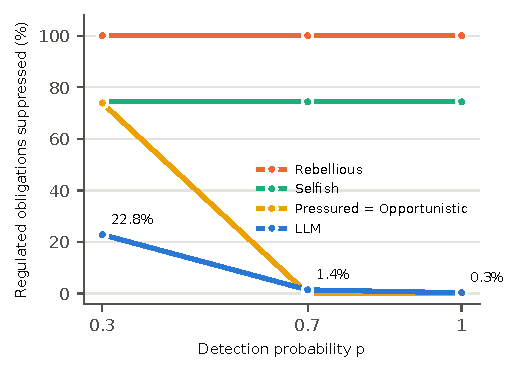
\includegraphics[width=\columnwidth]{figures/viana9.pdf}
\caption{Share of regulated alarm obligations suppressed as a function of the detection probability (default sanction; mean of 3 seeds). With the default sanction, pressured and opportunistic agents behave identically. The LLM responds to enforcement like them but violates a much smaller share.}
\label{fig:9}
\end{figure}

Selfish agents ignored enforcement: about 175 suppressions per run at every detection level and sanction scale. Opportunistic agents responded only to detection: they violated at p = 0.3 and complied at p $\geq$ 0.7, whatever the sanction. Pressured agents responded to the expected punishment: with the default sanction they violated at p = 0.3 and complied at p $\geq$ 0.7; with a sanction three times larger they complied even at p = 0.3; with a sanction five times smaller they violated at every detection level. The LLM suppressed 53.7, 3.3 and 0.7 alarms per run at p = 0.3, 0.7 and 1.0—22.8\%, 1.4\% and 0.3\% of its regulated obligations (Fig.~\ref{fig:9}). Its response to enforcement therefore has the shape of the pressured and opportunistic strategies, which make the same prediction under the default sanction; because the LLM was run only with that sanction, our design cannot tell which of the two it resembles more, and its justifications cite both the sanction (38\% of violations) and the detection probability (29\%).

The difference lies in the level. A pressured agent violates every obligation it believes false when the expected sanction is low: at p = 0.3, suppressing yields satisfaction 3, against an expected sanction of 0.3 $\times$ 5 = 1.5 and the lost reward of 1. The LLM often reasoned in the same terms (``the expected cost of the sanction, 0.3 $\times$ 5 = 1.5, is acceptable''), but it also priced a risk the pressured strategy ignores: that its belief could be wrong. If a real deterioration costs 20, suppressing pays off only when the probability that the alarm is real is below 2.5\%, and the LLM said so explicitly (``since harm costs 20, against a net gain of about 2 for not sounding, a low probability of real deterioration is enough to justify the alarm''; quotations translated from Portuguese). Such reasoning is a rational response to uncertainty, but it was conservative relative to the LLM's own accuracy: of the 434 obligations it believed false at p = 0.3 (three seeds), only 1 was a real deterioration. Experienced sanctions did not deter it either: among obligations it believed false at p = 0.3, it violated 28\% before its first detected sanction (n = 43) and 38\% afterwards (n = 391). This is consistent with the design—the detection probability is stated in the prompt, so a sanction carries no new information—but it means the normative record in the prompt did not act as a learning signal. \textbf{Answer to RQ6:} enforcement separated the classical strategies exactly as their definitions predict. The LLM responded to detection like a pressured or opportunistic agent, with a steep drop between p = 0.3 and p = 0.7, but it violated selectively and far below the level that expected-value reasoning on its own beliefs would justify.

\subsection{RQ7 – Are the LLM's violations justified and coherent?}\label{sec:5.3}
\begin{table*}[!t]
\centering
\caption{LLM deliberation by detection probability (3 seeds; mean $\pm$ s.d. per run where applicable). Belief sensitivity and specificity compare the stated belief (``the deterioration is real'') with the ground truth, recovered by replaying the transcripts.}
\label{tab:12}
\footnotesize
\setlength{\tabcolsep}{0.06cm}
\renewcommand{\arraystretch}{1.15}
\begin{tabular}{@{}>{\raggedright\arraybackslash}p{\dimexpr0.090\textwidth-0.12cm\relax}>{\raggedright\arraybackslash}p{\dimexpr0.140\textwidth-0.12cm\relax}>{\raggedright\arraybackslash}p{\dimexpr0.100\textwidth-0.12cm\relax}>{\raggedright\arraybackslash}p{\dimexpr0.110\textwidth-0.12cm\relax}>{\raggedright\arraybackslash}p{\dimexpr0.120\textwidth-0.12cm\relax}>{\raggedright\arraybackslash}p{\dimexpr0.120\textwidth-0.12cm\relax}>{\raggedright\arraybackslash}p{\dimexpr0.160\textwidth-0.12cm\relax}>{\raggedright\arraybackslash}p{\dimexpr0.160\textwidth-0.12cm\relax}@{}}
\hline
\textbf{Detection p} & \textbf{Suppressions} & \textbf{Share justified} & \textbf{Harmed episodes} & \textbf{Belief sensitivity} & \textbf{Belief specificity} & \textbf{Complied believing false} & \textbf{Violated believing real} \\ \hline
0.3 & 53.7 $\pm$ 12.5 & 1.000 & 0.0 $\pm$ 0.0 & 0.981 & 0.664 & 91.0 $\pm$ 8.5 & 0.0 $\pm$ 0.0 \\
0.7 & 3.3 $\pm$ 4.2 & 1.000 & 0.0 $\pm$ 0.0 & 1.000 & 0.689 & 146.3 $\pm$ 18.6 & 0.0 $\pm$ 0.0 \\
1 & 0.7 $\pm$ 1.2 & 1.000 & 0.0 $\pm$ 0.0 & 0.981 & 0.710 & 154.0 $\pm$ 8.2 & 0.0 $\pm$ 0.0 \\ \hline
\end{tabular}
\end{table*}

\textbf{Justification of violations.} All of the LLM's suppressions were justified at every detection level (share justified = 1.000): every alarm it suppressed was false, and it harmed no patient. Its stated beliefs were highly sensitive (0.981 at p = 0.3) but not specific (0.664): only in 2 of 2115 deliberations across all runs did it judge a real deterioration false—and in each case it complied anyway—whereas it judged about a third of the false alarms real. In Study 1, the LLM decision agent, asked only whether an alarm was real, had traded sensitivity for specificity; asked the same question as a deliberating agent that bears a harm penalty, the same model leaned toward caution. Stated beliefs thus depend on the role and incentives under which they are elicited.

\textbf{Coherence between belief and decision.} The LLM never violated an obligation while declaring the deterioration real, and it complied while declaring the alarm false in 91, 146 and 154 cases per run at p = 0.3, 0.7 and 1.0 (Table~\ref{tab:12}). Decision and belief are therefore coherent in the weak sense that no decision contradicts the stated belief. A stronger test is possible because the three detection levels share the same seeds, patients and alarms: the 705 obligations were decided under p = 0.3 and again under p = 1.0, with identical clinical evidence. If the beliefs were independent of the incentives, changes between the two conditions would be due to sampling noise and would be symmetric. They were not: 45 beliefs changed from ``real'' to ``false'' and only 15 from ``false'' to ``real'' (exact McNemar test, p = 0.0001). When suppressing was attractive (p = 0.3), the LLM more often declared the deterioration real—the belief that licenses compliance; when detection was certain and compliance was settled by the sanction, it declared the alarm false more freely and complied ``because the violation would be detected with certainty''. The stated belief follows the decision context, which indicates that the justification partly rationalizes the decision rather than reporting an independent clinical judgment.

\begin{table*}[!t]
\centering
\caption{Themes mentioned in the LLM's justifications, by decision (all 2,115 decisions of the nine runs; keyword coding in Portuguese and English, so a justification can mention several themes).}
\label{tab:13}
\footnotesize
\setlength{\tabcolsep}{0.06cm}
\renewcommand{\arraystretch}{1.15}
\begin{tabular}{@{}>{\raggedright\arraybackslash}p{\dimexpr0.250\textwidth-0.12cm\relax}>{\raggedright\arraybackslash}p{\dimexpr0.130\textwidth-0.12cm\relax}>{\raggedright\arraybackslash}p{\dimexpr0.155\textwidth-0.12cm\relax}>{\raggedright\arraybackslash}p{\dimexpr0.155\textwidth-0.12cm\relax}>{\raggedright\arraybackslash}p{\dimexpr0.155\textwidth-0.12cm\relax}>{\raggedright\arraybackslash}p{\dimexpr0.155\textwidth-0.12cm\relax}@{}}
\hline
\textbf{Theme mentioned} & \textbf{Violated (n = 173)} & \textbf{Complied, believed false, p = 0.3 (n = 273)} & \textbf{Complied, believed false, p = 0.7 (n = 439)} & \textbf{Complied, believed false, p = 1 (n = 462)} & \textbf{Complied, believed real (n = 768)} \\ \hline
Clinical evidence: trend or stability & 76\% & 57\% & 58\% & 56\% & 18\% \\
Clinical evidence: artifact or signal & 60\% & 62\% & 59\% & 54\% & 64\% \\
The norm or the obligation & 88\% & 75\% & 75\% & 73\% & 15\% \\
Detection or audit & 29\% & 20\% & 14\% & 92\% & 11\% \\
Sanction & 38\% & 8\% & 44\% & 63\% & 11\% \\
Harm or harm penalty & 12\% & 45\% & 56\% & 34\% & 26\% \\
Patient safety & 3\% & 63\% & 60\% & 53\% & 61\% \\
Alarm fatigue or satisfaction & 85\% & 55\% & 62\% & 65\% & 26\% \\
Uncertainty & 0\% & 38\% & 31\% & 21\% & 12\% \\ \hline
\end{tabular}
\end{table*}

\textbf{Content of the justifications.} Table~\ref{tab:13} shows what the LLM cited. Violations rested on clinical evidence that the alarm was false—stability of the trend (76\%), artifacts (60\%)—and on alarm fatigue (85\%); they rarely invoked patient safety (3\%) and never uncertainty, e.g., ``heart rate of 120 is within the usual range of this patient with chronic sinus tachycardia [\ldots{}]; not sounding avoids alarm fatigue; the expected cost of the sanction (0.3 $\times$ 5 = 1.5) is acceptable''. Compliance despite believing the alarm false was justified mainly by safety (63\% at p = 0.3), harm (45\%) and residual uncertainty (38\%); the share that cited the detection probability rose from 20\% at p = 0.3 to 92\% at p = 1.0, when certain detection became the stated reason to comply. Compliance with alarms believed real was justified almost only by clinical evidence and safety; incentives were rarely mentioned. Finally, 14\% of the justifications were written in English although every prompt was in Portuguese, a reminder that output conventions are not fully controlled by the prompt. \textbf{Answer to RQ7:} the LLM's violations were all justified ex post, and its decisions never contradicted its stated beliefs. Its beliefs, however, were cautious and moved with the enforcement level for identical evidence, so its justifications are informative about the factors it weighed but cannot be read as independent evidence about the patient.

\section{Implications}\label{sec:6}
\subsection{For LLM-driven norm adaptation}\label{sec:6.1}
Our results separate two claims that are easily conflated: that \emph{adaptive norms} help, and that \emph{LLMs} make adaptation better. The first was clearly supported—per-patient thresholds and persistence removed most false alarms without missed episodes. The second was not: a deterministic recommender did better. The LLM recommender's caution is understandable—its evidence mixed confirmed outcomes with unconfirmed verdicts without saying which was which—and suggests a concrete design rule for ANA-ML 2.0: evidence passed to an LLM-NormRecommender should carry its \emph{provenance} (confirmed outcome versus agent verdict). We also recommend that latency be reported alongside false alarms, since the two trade off, and that safety bounds remain deterministic, as in our validator.

\subsection{For LLM decision support}\label{sec:6.2}
Matching a validated clinical score is a meaningful but modest result. The LLM's distinctive contribution was not accuracy but explanation: each verdict came with a justification a clinician can check. Evaluations of LLM decision agents should therefore include a strong domain baseline and an explicit ceiling; without them, an accuracy of 0.8 is uninterpretable.

\subsection{For engineering LLM-based MAS simulations}\label{sec:6.3}
\begin{itemize}
\item Use synchronous rounds and seeded canonical message ordering; test order invariance explicitly.
\item Give every LLM component a deterministic counterpart and change one component per condition.
\item Never let observations encode the ground truth; model noise explicitly and report a ceiling.
\item Define protocol commands so that mentioning a command is distinguishable from issuing it, and give agents feedback when an action has no effect.
\item Make obligations count only effective actions; decide explicitly whether they re-arm.
\item Pair results by seed, censor unfinished runs, and treat any single API failure as recoverable.
\item Estimate cost with a dry run before spending, and keep full transcripts for auditing.
\end{itemize}

\subsection{The auditor as a transparency mechanism}\label{sec:6.4}
The LLM-NormAuditor was the most useful LLM component in practice. In an early run it identified a real measurement defect (Table~\ref{tab:8}, \#2). In the final run it also raised a false suspicion—three metrics with identical values, which we verified to be an arithmetic coincidence—showing that its reports are valuable prompts for human inspection rather than verdicts.

\subsection{Deviating from norms versus adapting them}\label{sec:6.5}
Study 2 suggests that autonomy over compliance is a lever comparable to norm adaptation—and, offline, a stronger one—provided two design conditions hold. First, safety-critical norms must be regimented: every harm we observed was bounded by the critical norm, which no strategy could violate. Second, incentives must keep individual satisfaction aligned with social contribution. With our a priori values they did (rebellion was the least satisfying strategy), but the balance depends on the harm penalty and on enforcement, and must be checked whenever they change.

\subsection{For LLM deliberation in ANA-ML 2.0}\label{sec:6.6}
The LLM was a \emph{safe} deliberative agent: under a regimented safety norm and an explicit harm penalty, it violated only alarms that were false and never delayed the recognition of a deterioration. It was not an \emph{effective} one: its caution left most of the alarm fatigue in place, and it used its own accurate beliefs far less than expected-value reasoning would allow. For regulated, non-critical norms with a regimented safety net, delegating compliance decisions to an LLM is therefore defensible, but it should not be expected to outperform a well-calibrated deterministic rule. Three design rules follow for ANA-ML 2.0 and JSAN:

\begin{itemize}
\item \textbf{Separate Analyze from Decision.} ANA-BDI already distinguishes the stage that forms judgments from the stage that chooses (Fig.~\ref{fig:1}). Our results show why this separation should be kept when an LLM fills the deliberation hot spot: when one call both judges the alarm and decides, the stated belief follows the incentive. Beliefs should be elicited in a call that does not see rewards, sanctions or detection probabilities, and the decision should consume them.
\item \textbf{Audit justifications counterfactually.} A justification is a useful account of the factors the model weighed, but not independent evidence. Auditors such as the LLM-NormAuditor should compare decisions on the same evidence under different incentives—as our paired design did—rather than assess each justification on its own.
\item \textbf{Make calibration explicit.} The LLM priced the harm penalty correctly in words but acted as if its beliefs were less reliable than they were. Feeding back confirmed outcomes of its own suppressions did not change its behavior; giving it calibrated probabilities, or applying a deterministic expected-value rule to its stated beliefs, are alternatives worth testing.
\end{itemize}

\section{Threats to Validity}\label{sec:7}
\textbf{Construct validity.} The ICU scenario is synthetic: physiology is reduced to Gaussian vital signs with linear deterioration, and the bedside-findings model and its probabilities were designed by the authors. The decision baseline is a modified NEWS2 score, not the official instrument. The marketplace and project scenarios are small and stylized.

\textbf{Internal validity.} We used a single model, at a single effort level, with one run per seed; LLM outputs are stochastic and prompt-sensitive, and other prompts could change the results. The heuristic baselines differ in strength across scenarios (weak in the marketplace, strong in project management). Engineering defects were mitigated by the controls in Table~\ref{tab:8} and by 78 automated tests, including order-invariance and no-leakage tests, but further defects cannot be excluded.

\textbf{Study 2.} The compliance strategies are our operationalizations of qualitative definitions \cite{lopez2002constraining}; the Motivation, Satisfaction, reward, sanction and harm values were fixed a priori and other values could change the balance between strategies; and the NEWS2-based belief used by the offline strategies was never wrong about real deteriorations in this scenario, which favors them. Each obligation is decided once, and obligations suppressed in the last two iterations never expire. The LLM was run only with the default sanction, so pressured and opportunistic behavior cannot be distinguished for it, and with one run per seed and detection level, so its sampling variability is confounded with the seed. The analysis of belief changes treats the decisions on each obligation as paired observations; decisions within a run are not fully independent, since the prompt carries the agent's normative record. The themes in Table~\ref{tab:13} were coded by keywords, not by human annotators, and are indicative only.

\textbf{External validity.} Results concern one LLM, three scenarios and simulated data; they should not be generalized to real clinical settings or to other models without replication.

\textbf{Conclusion validity.} With three paired seeds, no difference can reach conventional significance (minimum exact p = 0.25), and effect sizes are imprecise. We therefore report all findings as exploratory, together with per-seed data (Figs.~\ref{fig:4}--\ref{fig:5}).

\section{Concluding Remarks}\label{sec:8}
We presented a controlled, exploratory comparison of LLM-based and deterministic components in adaptive normative multi-agent systems. LLM agents negotiated better; adaptive norms reduced ICU false alarms; but an LLM did not improve norm recommendation or alarm triage over strong deterministic baselines, and adaptation increased latency. Building a fair comparison required controlling seventeen engineering threats to validity, two of which were revealed by the LLM-NormAuditor. In Study 2, agents decided whether to comply: well-informed deviation reduced false alarms more than norm adaptation, uninformed deviation harmed patients within the bounds of a regimented norm, and enforcement separated the classical strategies as predicted. The LLM deliberative agent was safe but conservative: it suppressed 23\% of regulated alarms when detection was unlikely and almost none when it was certain, all of them false, and harmed no patient; yet its stated beliefs shifted with the detection probability for identical evidence, so its justifications partly rationalize its decisions. As future work, we plan to (i) replicate both studies with more seeds, other models and effort levels; (ii) give the recommender label provenance; (iii) evaluate the LLM validator as a separate condition; (iv) separate belief elicitation from the compliance decision and run the LLM under several sanction sizes; (v) study populations of deliberative agents and the canonical ANA rescue scenario; and (vi) validate the approach on real data. The platform, data and transcripts are available in the \emph{llm-mas} repository [link to be added].

\section*{Acknowledgment}
[Funding: CAPES, CNPq and NSERC, to be confirmed.] [Disclosure of AI assistance in software development and drafting, according to the venue's policy.]


\bibliographystyle{IEEEtran}
\bibliography{IEEEabrv,references}

% Biografias copiadas do modelo ANA-ML 2.0 (access (2).tex); as fotos devem estar nesta pasta.
\begin{IEEEbiography}[{\includegraphics[width=1in,height=1.5in,clip,keepaspectratio]{marx_viana_pb.png}}]{Marx Viana} received a B.S. in computer science from Federal University of Viçosa (UFV), in 2010, and the Master's in Informatics and Ph.D. degrees at the Pontifical Catholic University of Rio de Janeiro (PUC-RJ), in 2012 and 2016, respectively.

He is a currently a researcher at PUC-RJ. His research in computer science span a wide range of topics with an emphasis on software engineering, and focus on software frameworks, object-oriented design and programming, software agents, software adaptation, and normative systems.
\end{IEEEbiography}

\begin{IEEEbiography}[{\includegraphics[width=1in,height=1.25in,clip,keepaspectratio]{elder-menino.jpg}}]{Elder Cirilo} received a B.S. in Computer Science from Federal University of Juiz de Fora (UFJF), in 2006, and the Master's and Ph.D. degrees in Informatics at the Pontifical Catholic University of Rio de Janeiro (PUC-RJ), in 2008 and 2012, respectively. He has been an Assistant Professor in the Department of Computer Science at the Federal University of São João del Rei since 2013.

He has experience in the area of software engineering, with an emphasis on the following themes: configurable software systems, domain specific languages, feature-oriented software development, end-user programming and experimental software engineering.
\end{IEEEbiography}

\begin{IEEEbiography}[{\includegraphics[width=1in,height=1.25in,clip,keepaspectratio]{palencar.png}}]{Paulo Alencar} is a Research Professor with the David R. Cheriton School of Computer Science at the University of Waterloo, and Associate Director of the Computer Systems Group (CSG).

Dr. Alencar has received international research awards from organizations such as Compaq and IBM. He has published over 250 refereed publications and has been a member of program committees of numerous highly-regarded conferences and workshops. His recent research in information technology and software engineering has focused on high-level software architectures, design, components and their interfaces; software frameworks and application families; software processes, automated workflows and work graphs, and evolution; web-based approaches and applications; open and big data applications; context-aware and event-based systems; software agents;
machine learning; cognitive chatbots; artificial intelligence; and formal
methods. He has been Principal or Co-Principal Investigator in projects
supported by NSERC, ORF-RE, IBM, SAP, CITO, CSER, Bell, and funding agencies in Canada U.S., Brazil, Germany and Argentina. He is a member of the Association of Computing Machinery (ACM), Institute of Electrical and Electronic Engineers (IEEE), Association for the Advancement of Artificial Intelligence (AAAI), Waterloo Water Institute (part of the Global Water Futures initiative), and Waterloo Artificial Intelligence Institute.
\end{IEEEbiography}

\begin{IEEEbiography}[{\includegraphics[width=1in,height=1.25in,clip,keepaspectratio]{don_cowan.jpeg}}]{Don Cowan} (Life Member, IEEE) is currently a Distinguished Professor Emeritus of computer science with the University of Waterloo and the Director of the Computer Systems Group. He has made contributions to computer science in areas, such as computer science, software engineering, and complex applications. He is the author and coauthor or an editor of over 300 refereed articles and 17 books in computer/communications, software engineering, education, environmental information systems, and mathematics. He has supervised over 120 graduate students and postdoctoral fellows. His group has developed over 80 Web-based and mobile software systems for many application areas. The University of Waterloo recognized his contributions to development of graduate students by presenting him with the Award of Excellence in Graduate Supervision. He was recognized for his research and support of the development of computer science in Brazil by being awarded the National Order of Scientific Merit (Grand Cross), the country's highest civilian scientific honour, by the President of Brazil. In 2009, he received the Waterloo Award, the City of Waterloo's highest civic honour, for his contributions to the City of Waterloo. In 2010, he was named a Distinguished Scientist by the Association for Computing Machinery. In 2011, he received a Doctor of Science (Honoris Causa) from the University of Guelph for his contributions to Computer Science and Software Engineering.
\end{IEEEbiography}

\begin{IEEEbiography}[{\includegraphics[width=1in,height=1.25in,clip,keepaspectratio]{carlos_lucena.jpeg}}]{Carlos Lucena} received a BSc degree from the Pontifical Catholic University of Rio de Janeiro (PUC-Rio), Brazil, in 1965,
a Math degree in computer science from the University of Waterloo, Canada, in 1969, and a PhD degree in computer science from the University of California at Los Angeles in 1974. He has been a full professor in the Department of Informatics at PUC-Rio
since 1982.

Dr. Carlos Lucena has made extensive and internationally recognized research contributions, being the author or co-author of over 600 refereed papers and 19 books in the area of software design and formal methods in software
engineering, his primary areas of research. He has also been a member of the program committees of more than
62 national and international conferences as well as member of the editorial board of some important journals in his area of research. Until 2015, he has supervised 45 PhD theses and 114 M.Sc. dissertations. His former PhD students are faculty members in universities in Brazil and abroad (e.g., USA and Canada). He is also a member of
the Editorial Board of the International Journal on Formal Aspects of Computing (New York: Springer-Verlag).
He worked at the Pontifical Catholic University of Rio de Janeiro as vice-rector of the University, Dean for the Center for Science and Technology, and several times as Director of the Computer Science Department. Prof.
Lucena was awarded the insignia for the Grand Cross of the Order of Scientific Merit of the Presidency of the
Republic of Brazil, the Medal of Scientific Merit Carlos Chagas Filho from the Council of Directors of FAPERJ (State Research Council), the Alvaro Alberto Award for Science and Technology (Ministry of Science and Technology)
and several times the IBM Innovation Award, among many others. Prof. Lucena is a Fellow of the Guggenheim
Foundation, an ACM Fellow and a member of the Brazilian Academy of Sciences.
\end{IEEEbiography}


\EOD

\end{document}
